
\documentclass{beamer}

\mode<presentation> {


\usetheme{Montpellier}

% As well as themes, the Beamer class has a number of color themes
% for any slide theme. Uncomment each of these in turn to see how it
% changes the colors of your current slide theme.

\usecolortheme{beaver}


%\setbeamertemplate{footline} % To remove the footer line in all slides uncomment this line
\setbeamertemplate{footline}[page number] % To replace the footer line in all slides with a simple slide count uncomment this line

\setbeamertemplate{navigation symbols}{} % To remove the navigation symbols from the bottom of all slides uncomment this line
}

\usepackage{graphicx} % Allows including images
\usepackage{booktabs} % Allows the use of \toprule, \midrule and \bottomrule in tables
\usepackage{amsmath}
\usepackage{lmodern}% http://ctan.org/pkg/lm
\newenvironment{where}{\noindent{}where\begin{itemize}}{\end{itemize}}
\DeclareMathOperator{\Exists}{\exists}
%----------------------------------------------------------------------------------------
%	TITLE PAGE
%----------------------------------------------------------------------------------------

\title[Exit Exam]{Fast Dictionary Attacks on Passwords Using Time-Space Tradeoff} % The short title appears at the bottom of every slide, the full title is only on the title page

\author{Tyler Combs} % Your name
\institute[OU] % Your institution as it will appear on the bottom of every slide, may be shorthand to save space
{
The University of Oklahoma \\ % Your institution for the title page
\medskip
\textit{tyler.combs@ou.edu} % Your email address
}
\date{April 14, 2015} % Date, can be changed to a custom date

\begin{document}

\begin{frame}
\titlepage % Print the title page as the first slide
\end{frame}

\begin{frame}
\frametitle{Overview} % Table of contents slide, comment this block out to remove it
\tableofcontents % Throughout your presentation, if you choose to use \section{} and \subsection{} commands, these will automatically be printed on this slide as an overview of your presentation
\end{frame}

%----------------------------------------------------------------------------------------
%	PRESENTATION SLIDES
%----------------------------------------------------------------------------------------

%------------------------------------------------
\section{Introduction} 
%------------------------------------------------
\subsection{Introduction}


\begin{frame}
\frametitle{Introduction}
\begin{itemize}
\item Humans tend to generate passwords that are easy to remember
\item Common defense: \emph{composition rules} require passwords to include digits and special characters
\item Even with the addition of digits and special characters, Humans are not too random
\end{itemize}
\end{frame}

\begin{frame}
\frametitle{Introduction}
\begin{itemize}
\item Consider a string ``abababababababab'' 16 characters long
\item Although the string is long and hard to brute-force, is is not very random
\item This can be modeled by the \emph{Kolmogrov conplexity} (K-Complexity)
\begin{itemize}
\item Kolmogrov complexity: The length of the shortest Turing Machine that outputs a string and then haults
\end{itemize}
\end{itemize}
\end{frame}

\begin{frame}
\frametitle{Introduction}
\begin{itemize}
\item Itterate over all strings with K-Complexity $\leq$ some threshold
\item Can't be done
\begin{itemize}
\item K-Complexity is uncomputable
\item Human randomness is different than computational randomness
\end{itemize}
\item Solution: Use techniques from natural language processing, such as ``Markovian Filters'' to generate strings that are phonetically simmilar to the users natural language
\end{itemize}
\end{frame}


\begin{frame}
\frametitle{Goal}
Ultimate goal: given a cipher text $c$ recover the password $k$ such that $H(k) = c$
\end{frame}

\subsection{Time-Space Tradeoff}
\begin{frame}
\frametitle{Time-Space Tradeoff}



\begin{columns}[c] % The "c" option specifies centered vertical alignment while the "t" option is used for top vertical alignment
\column{.30\textwidth} % Left column and width
Full look up table \\
\begin{block}{Time}
$O(1)$
\end{block}

\begin{block}{Space}
$O(\lvert \mathcal{K} \rvert)$
\end{block}
\column{.30\textwidth} % Right column and width
?????


\column{.30\textwidth} % Right column and width
Brute-force attack \\
\begin{block}{Time}
$O(\lvert \mathcal{K} \rvert)$
\end{block}

\begin{block}{Space}
$O(1)$
\end{block}
\end{columns}
\end{frame}




\begin{frame}
\frametitle{Time-Space Tradeoff}
\begin{columns}[c]
\column{.50\textwidth}
In 1980 Martin Hellman answes this question by contributing a Time-Space tradeoff for the problem of cryptanalysis.
\begin{itemize}
\item Precompute: $m$ ``chains'' of length $t$
\item Store only the first and last items in each chain
\end{itemize}
\column{.45\textwidth}
\begin{figure}
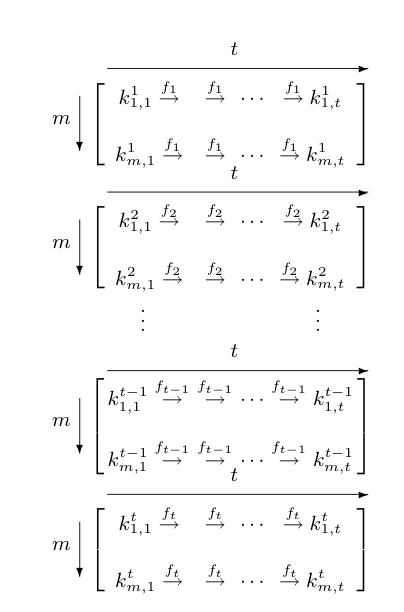
\includegraphics[width=0.9\linewidth]{figs/classic}
%\caption{Convergence vs reduction in Keyspace size ($|\mathcal{K}|$) for 8-character sequences}
\end{figure}
\end{columns}
\end{frame}

\begin{frame}
\frametitle{Chain Generation}
\begin{columns}[c]
\column{.50\textwidth}
The function $f(k)$ maps from one key to another. Where:
\begin{equation*}
f(k) = R[H(k)]
\end{equation*}
\begin{where}
\item $H(k)$ is a hash function that maps from key $k$ to ciphertext $c$
\item $R(c)$ is a Reduction function mapping from a ciphertext $c$ back to a value $k \in \mathcal{K}$
\item Example reduction function: drop last n characters/bits
\end{where}
\column{.45\textwidth}
\begin{figure}
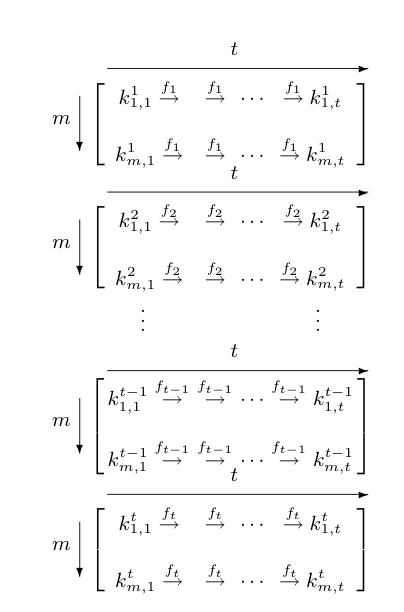
\includegraphics[width=0.9\linewidth]{figs/classic}
%\caption{Convergence vs reduction in Keyspace size ($|\mathcal{K}|$) for 8-character sequences}
\end{figure}
\end{columns}
\end{frame}


\begin{frame}
\frametitle{Chain Generation}
\begin{columns}[c]
\column{.50\textwidth}
\begin{example}[Chain Generation]
4-character passwords \\
6-character password sets
\begin{align*}
pass & \rightarrow^H FE4gT6 \rightarrow^R ofie \rightarrow^H \\ & FP03u2 \rightarrow^R ueyf \dotsb \rightarrow^R lswq
\end{align*}
\end{example}
\column{.45\textwidth}
\begin{figure}
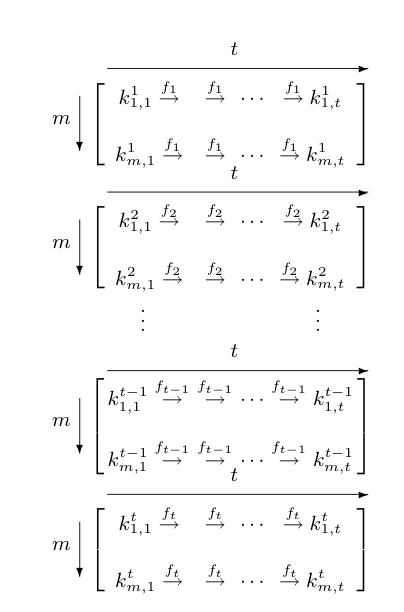
\includegraphics[width=0.9\linewidth]{figs/classic}
%\caption{Convergence vs reduction in Keyspace size ($|\mathcal{K}|$) for 8-character sequences}
\end{figure}
\end{columns}
\end{frame}



\begin{frame}
\frametitle{Key Recovery}
\begin{columns}[c]
\column{.50\textwidth}
\begin{itemize}
\item Given any cipher text $c$, use the reduction function $R$ to generate a key $k_i$
\item Generate a new chain of length $t$ (where $t$ is the length of chains in the stored table)
\item Search the \emph{last} elements of the precomputed table for every key generated from the given ciphertext $c$
\end{itemize}
\column{.45\textwidth}
\begin{figure}
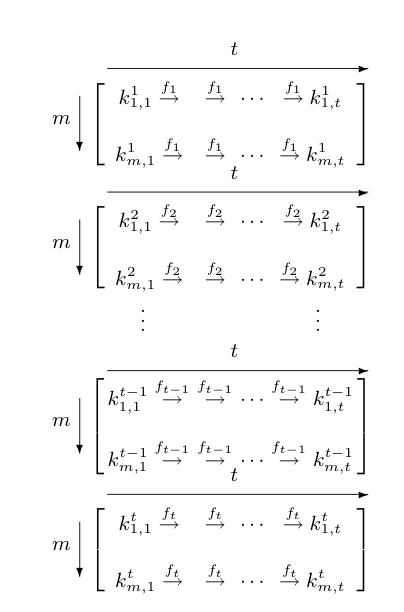
\includegraphics[width=0.9\linewidth]{figs/classic}
%\caption{Convergence vs reduction in Keyspace size ($|\mathcal{K}|$) for 8-character sequences}
\end{figure}
\end{columns}
\end{frame}

\begin{frame}
\frametitle{Key Recovery}
\begin{columns}[c]
\column{.50\textwidth}
\begin{itemize}
\item Because we found the chain our ciphertext belongs to, we can recover the key that generates the ciphertext
\item Time-Space Tradeoff comes from the length of the chains
\end{itemize}

\begin{example}[On Board]

\end{example}
\column{.45\textwidth}
\begin{figure}
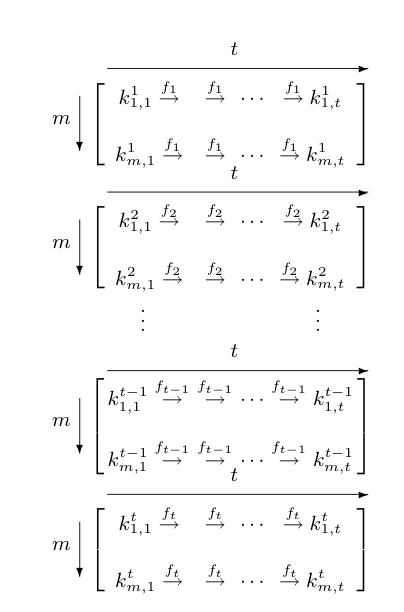
\includegraphics[width=0.9\linewidth]{figs/classic}
%\caption{Convergence vs reduction in Keyspace size ($|\mathcal{K}|$) for 8-character sequences}
\end{figure}
\end{columns}
\end{frame}


\begin{frame}
\frametitle{Problem}
Chains can merge. The reduction function can produce the same key for two different ciphertexts
\begin{itemize}
\item If the merge happens early in the chain generation, the table will not cover as many passwords
\item Hard to detect because the chains will still have different end points (Unless the merge happens at the same position in the two chains)
\end{itemize}
\end{frame}

\begin{frame}
\frametitle{Solution}
\textbf{Rainbow Tables}
\begin{itemize}
\item Use different related reduction functions $R_1$ to $R_n$ where $n$ is the length of the chain
\item If a collision happens, It has to be at the same position in chain generation and collisions can be detected
\item Key recovery changes because we are using a different reduction function each time.
\begin{itemize}
\item assume generate chain starting at position $n-1$ use reduction function $R_{n-1}$ and move backwards through the chain
\end{itemize}
\end{itemize}
\end{frame}

\subsection{Smart Dictionary Attack}
\begin{frame}
\frametitle{Smart Dictionary Attacks}
\begin{itemize}
\item Rainbow tables and the classical space-time tradeoff make \textbf{no assumptions} about the keyspace other than its size
\item Narayanan and Shmatikov use Markov chains and Regular expressions to make some assumptions about the keyspace. This means that we can search only a ``smart'' portion of the keyspace.
\end{itemize}
\end{frame}

%------------------------------------------------
\section{Filtering} 
%------------------------------------------------
\subsection{Markovian}

\begin{frame}
\frametitle{Markov Chains}
\begin{itemize}
\item Markov chains are commonly used in natural language processing. Most notably speech recognition systems.
\item Markov models have been used to generate passwords for users.
\item Given a set of states $S = \lbrace s_1,s_2,\dotsb,s_n \rbrace$ there is some probability $p_{ij}$ that denotes the probability of transitioning from state $s_i$ to state $s_j$
\item The probability of transitioning to the next state depends only on the current state
\end{itemize}
\end{frame}

\begin{frame}
\frametitle{Markov Chains}

\textbf{The order of a Markov chain of order n is defined as:}
\begin{align*}
& P(X_n = x_n | X_{n-1} = x_{n-1}, X_{n-2} = x_{n-2}, \dotsb , X_1 = x_1) = \\ & P(X_n = x_n | X_{n-1} = x_{n-1}, \dotsb , X_{n-m} = x_{n-m})
\end{align*}

\textbf{Zero-order Markov Chain:}
\begin{align*}
& P(X_n = x_n | X_{n-1} = x_{n-1}, X_{n-2} = x_{n-2}, \dotsb , X_1 = x_1) =  \\ & P(X_n = x_n)
\end{align*}

\textbf{First-order Markov Chain:}
\begin{align*}
& P(X_n = x_n | X_{n-1} = x_{n-1}, X_{n-2} = x_{n-2}, \dotsb , X_1 = x_1) = \\ & P(X_n = x_n | X_{n-1} = x_{n-1})
\end{align*}
\end{frame}

\begin{frame}
\frametitle{Zero-order Markov Model}
In a zero-order Markov model, each character is generated given its underlying proability distribution. This is based on the frequency of the letter in the users natural language. Formally the zero-order model can be written as:
\begin{equation*}
P(\alpha) = \prod_{x \in \alpha} \mathcal{V}(x)
\end{equation*}
where:
\begin{where}
\item $P(\cdot)$ is the markovian proability distrubuion
\item $\alpha$ is a string of characacters
\item $\mathcal{V(\cdot)}$ is the frequency of a letter occuring in English
\item $x$ is an individual character
\end{where}
\end{frame}


\begin{frame}
\frametitle{First-order Markov Model}

In a First-order Markov model, each ordered pair is assigned a proability and each character is generated by looking at the pervious character. The first-order markov model can be written as:
\begin{equation*}
P(x_1x_2x_3 \dotsb x_n) = \mathcal{V}(x_1)\prod_{i=1}^{n-1}\mathcal{V}(x_{i+1}|x_i)
\end{equation*}
where:
\begin{where}
\item $P(\cdot)$ is the markovian proability distrubuion
\item $x_i$ are individual characters
\item $\mathcal{V(\cdot)}$ is the frequency of a letter or ordered pair occuring in English
\end{where}
\end{frame}



\begin{frame}
\frametitle{Markov Dictionary}
A probability distribution is not a dictionary. To create a dictionary, discretize the probabilities into two levels using a threshold $\theta$
\begin{block}{Zero-order dictionary}
\begin{equation*}
\mathcal{D}_{\mathcal{V},\theta} = \lbrace \alpha : \prod_{x \in \alpha}\mathcal{V}(x) \geq \theta \rbrace
\end{equation*}
\end{block}

\begin{block}{First-order dictionary}
\begin{equation*}
\mathcal{D}_{\mathcal{V},\theta} = \lbrace x_1x_2 \dotsb x_n : \mathcal{V}(x_1) \prod_{i = 1}^{n-1} \mathcal{V}(x_{i+1}|x_i) \geq \theta \rbrace
\end{equation*}
\end{block}
\end{frame}

\begin{frame}
\frametitle{Markov Dictionary}
The zero-order model is better for abrivtations and acrynyms. For example, a user picks their favorite song lyric and the first letter of each word creates their password.
\begin{figure}
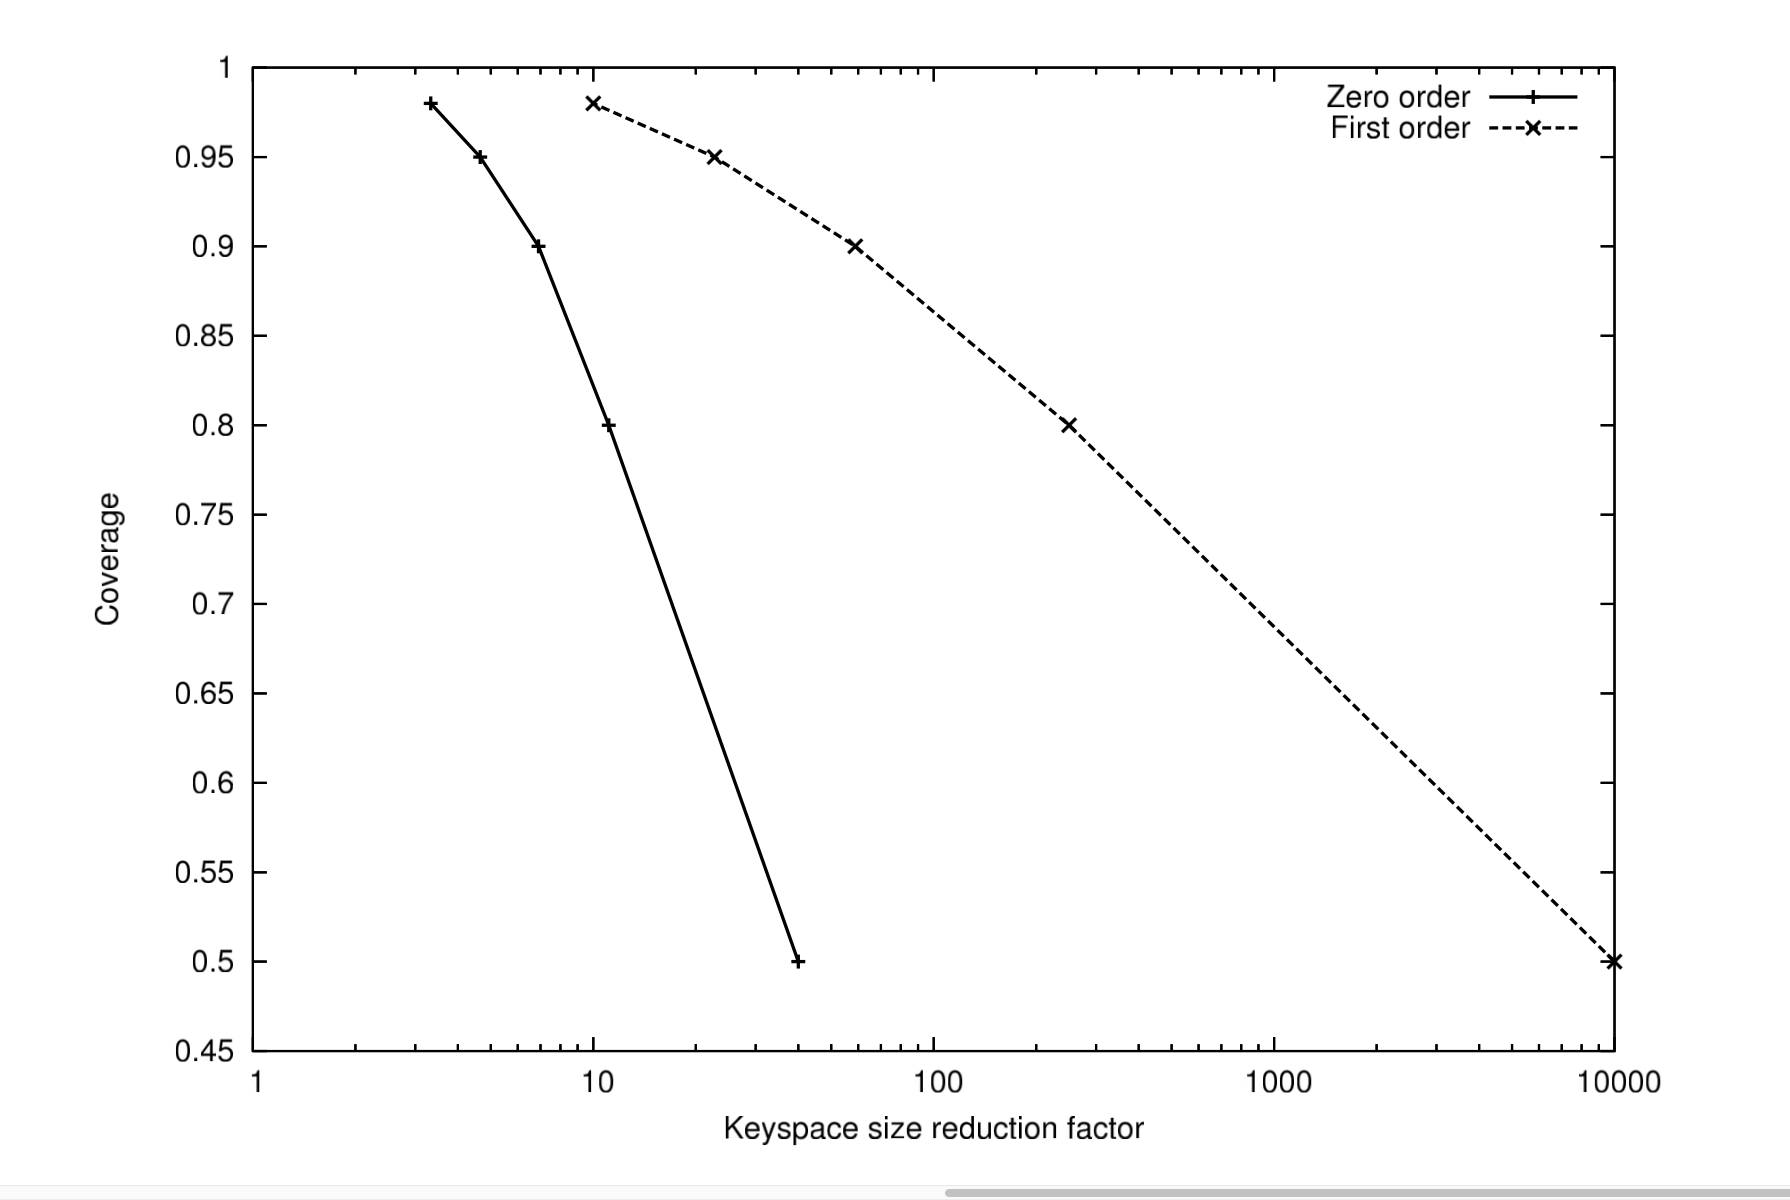
\includegraphics[width=0.6\linewidth]{figs/dict_plot}
\caption{Convergence vs reduction in Keyspace size ($|\mathcal{K}|$) for 8-character sequences}
\end{figure}
\end{frame}

\subsection{Finite Automaton}
\begin{frame}
\frametitle{Deterministic Finite Automaton}
\begin{itemize}
\item A DFA or Deterministic Finite Automaton is a finite state machine that accepts or rejects a string
\item A regular expression can be constructed from a DFA
\item Humans are not random with how they use numerals and special characters
\begin{itemize}
\item Numbers tend to be at the end of a password: password1
\item Capital letters are typically at the begining of a password: Password
\item there are typically more lowercase letters in passwords than uppercase letters, numerals, or special characters
\end{itemize}
\end{itemize}
\end{frame}

\begin{frame}
\frametitle{Dictionary using a DFA} 
An improved dictionary is one where strings are both accepted by a Markovian filter and accepted by at least one DFA from some set of DFA's. The updated dictionary is defined as:
\begin{equation*}
\mathcal{D}_{\mathcal{V},\theta,\langle M_i \rangle} = \lbrace \alpha : \prod_{x \in \alpha}\mathcal{V}(x) \geq \theta, and \Exists i : M_i accepts \alpha \rbrace
\end{equation*}
\begin{where}
\item $A$ is the set of 26 uppercase characters
\item $a$ is the set of 26 lowercase characters
\item $n$ is the set if 10 numerals
\item $s$ is the set of 5 special characters $\lbrace space, hyphen, underscore, period, comma \rbrace$
\end{where}

\end{frame}

%------------------------------------------------
\section{Indexing Algorithms} 
%------------------------------------------------
\begin{frame}
\frametitle{Indexing Algorithms}
\begin{itemize}
\item The goal is to create an algorithm that will efficiently enumerate the passwords in a given password space. Given $i$ as input return the $i^{th}$
\item In the rainbow attack the reduction function maps from ciphertext space to $\lbrace 0, 1, \dotsb, \lvert \mathcal{K} - 1 \rvert \rbrace$
\item Composed with a mapping from $\lbrace 0, 1, \dotsb, \lvert \mathcal{K}-1 \rvert \rbrace$ to a key in $\mathcal{K}$.
\item Makes no assumption about keyspace other than its size
\item Use the rainbow attack with a "smart" way to choose the keyspace
\end{itemize}
\end{frame}

\begin{frame}
\frametitle{Dictionary Modification}
Modify the dictionary to only consider fixed length strings. This allows for different threshold values $\theta$ for each length.
\begin{equation*}
\mathcal{D}_{\mathcal{V},\theta,\ell} = \lbrace \alpha :  \lvert \alpha \rvert = \ell and \prod_{x \in \alpha}\mathcal{V}(x) \geq \theta \rbrace
\end{equation*}
\end{frame}

\begin{frame}
\frametitle{Discretization}
The algorithm also needs to discretize the probability distribution of the strings. First, turn the dictionary into a sum rather than a product. \\
Transform the product
\begin{align*}
\prod_{x \in \alpha}\mathcal{V}(x) & \geq \theta \\
\log(\prod_{x \in \alpha}\mathcal{V}(x)) & \geq \log(\theta) \\
\log(\mathcal{V}(x_1)\mathcal{V}(x_2)\dotsb \mathcal{V}(x_n)) & \geq \log(\theta) \\
\log(\mathcal{V}(x_1)) + \log(\mathcal{V}(x_2)) + \dotsb + log(\mathcal{V}(x_n)) & \geq \log(\theta)
\end{align*}
\end{frame}

\begin{frame}
\frametitle{Discretization}
To arrive at a discrete version of the modified dictionary:
\begin{equation*}
\mathcal{D}_{\mathcal{V},\theta,\ell} = \lbrace \alpha :  \lvert \alpha \rvert = \ell and \sum_{x \in \alpha}\mu(x) \geq \lambda \rbrace
\end{equation*}
Where
\begin{where}
\item $\mu(x) = \log(\mathcal{V}(x))$
\item $\lambda = \log(\theta)$ 
\end{where}
\end{frame}

\begin{frame}
\frametitle{Discretization}
\begin{itemize}
\item $\mu(x) = \log(\mathcal{V}(x))$
\item Discretize the values of the $\mu$ function to the nearest multiple of some $\mu_0$
\item Narayanan and Shmatikov use a $\mu_0$ that yields approximately 1000 different discrete values
\end{itemize}
\end{frame}


\begin{frame}
\frametitle{Partial Dictionary}
Define a partial dictionary $\mathcal{D}_{\mathcal{V},\theta,\ell,\theta^\prime,\ell^\prime}$ as follows:
\begin{itemize}
\item let $\alpha$ be a string such that $\lvert \alpha \rvert = \ell^\prime$
\item $\prod_{x \in \alpha}\mathcal{V}(x)=\theta^\prime$ 
\end{itemize} 
Then
\begin{equation*}
\mathcal{D}_{\mathcal{V},\theta,\ell,\theta^\prime,\ell^\prime} = \lbrace \beta : \alpha \beta \in \mathcal{D}_{\mathcal{V},\theta,\ell} \rbrace
\end{equation*}
\end{frame}

\begin{frame}
\frametitle{Zero-Order Markovian Dictionary}
Precompute the size of a partial dictionary (recursively) and store in a 2D-array of size ($\ell$ , \texttt{num\_levels}) \\
\begin{equation*}
\lvert \mathcal{D}_{\mathcal{V},threshold, total\_length, level, current\_length} \rvert
\end{equation*}
\end{frame}

\begin{frame}[fragile]
\frametitle{Zero-Order Markovian Dictionary}
\begin{verbatim}
partial_size1(current_length, level)
{
    if level >= threshold: return 0
    if total_length = current_length: return 1
    sum = 0
    for each char in alphabet
        sum = sum + partial_size1(current_length+1, 
                                    level+mu(char))
    return sum
}
\end{verbatim}
Complexity linear in the product of total length, number of characters in alphabet, and number of levels
\end{frame}

\begin{frame}
\frametitle{Zero-Order Markovian Dictionary}
\begin{itemize}
\item For cryptanalysis, given an index $i$ produce the corresponding key $k$ in the dictionary $\mathcal{D}$
\item Use precomputed partial size to determine the first character by looking up a value from the precomputed matrix.
\begin{itemize}
\item Adjust the index to a new index relative to the first character
\item Adjust the threshold based on the frequency of the first character
\end{itemize}
\end{itemize}

\end{frame}

\begin{frame}[fragile]
\frametitle{Zero-Order Markovian Dictionary}
Initally call \texttt{get\_key1(0,0)}
\begin{verbatim}
get_key1(current_length, index, level)
{
    if total_length = current_length: return ""
    sum = 0
    for each char in alphabet
        new_level = level + mu(char)
        // looked up from precomputed array
        size = partial_size1[
            current_length+1][new_level]
        if sum + size > index
            return char + get_key1(
                current_length+1,
                index-sum, new_level)
        sum = sum + size
}
\end{verbatim}
\end{frame}

\begin{frame}
\frametitle{First-Order Markovian Dictionary}
Same as zero order only in get\_key, we need to keep track of the last character
\end{frame}

\begin{frame}
\frametitle{DFA Dictionary}
Similar to zero-order Markov dictionary except instead of a threshold and levels, we have states and transitions
\end{frame}

\begin{frame}
\frametitle{Any Keyspace $\mathcal{K}$}
Assume that we have a superspace $\mathcal{K}^\prime \supset \mathcal{K}$ ad we need to decide that given $\alpha \in \mathcal{K}^\prime$ if $\alpha \in \mathcal{K}$ \\
Split $\matcal{K}^\prime$ into $m$ bins of size $t$ and precompute the number of members in each bin that are in $\matcal{K}$ \\
Given an index, quickly figuew out what bin it falls into and interate over all keys in that bin and test each one for membership \\
$O(\lvert \matcal{K}^\prime \rvert)$ precomputation time 
... storage and index
\end{frame}

\begin{frame}
\frametitle{Hybrid Markovian/DFA}
\end{frame}

\begin{frame}
\frametitle{Multiple Keyspaces}
\end{frame}


%------------------------------------------------
\section{Experiment} 
%------------------------------------------------
\begin{frame}
\frametitle{Experiment}
\begin{itemize}
\item Measure coverage of rainbow attack vs hybrid attack
\item 142 real user passwords
\item 6-Character alphanumeric sequences for the rainbow attack ($|\mathcal{K}| = 36^6 \approx 2*10^9 $)
\item 70 regular expressions
\end{itemize}
\end{frame}

\begin{frame}
\frametitle{Results}
\begin{figure}
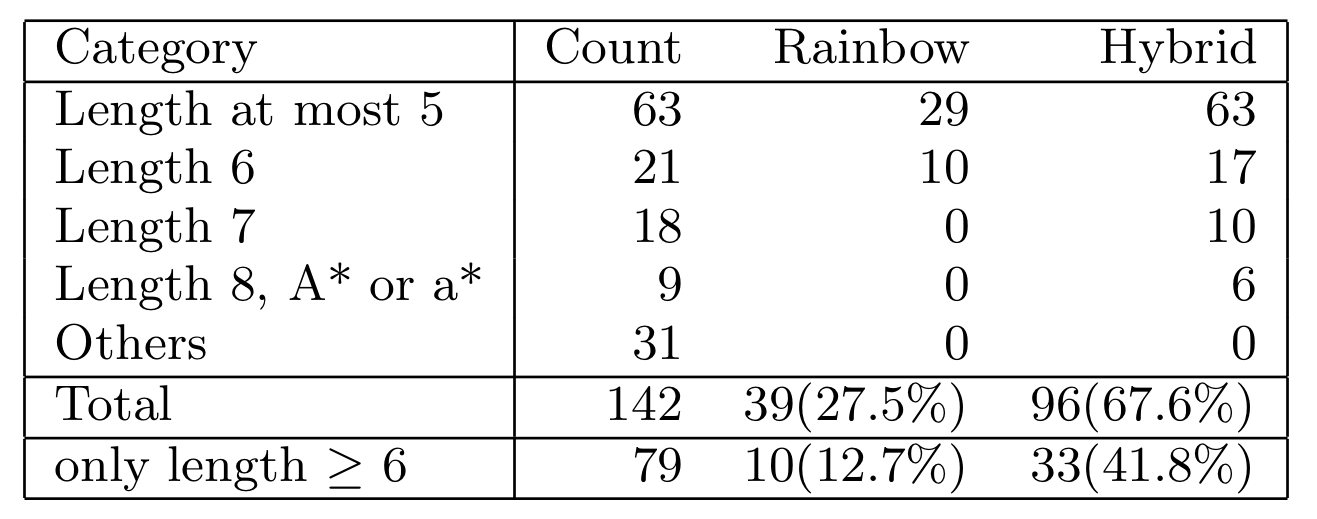
\includegraphics[width=0.9\linewidth]{figs/results}
\caption{Passwords recovered in Hybrid attack vs. Rainbow attack}
\end{figure}
\end{frame}

%------------------------------------------------
\section{Conclusions} 
%------------------------------------------------

\begin{frame}
\frametitle{Conclusions}
\begin{itemize}
\item One of many attacks targeting human weakness
\item Some possible defences against dictionary attacks for human memorable passwords
\begin{itemize}
\item Graphical passwords
\item Biometric information
\end{itemize}
\item Are these actually safer?
\end{itemize}
\end{frame}


%------------------------------------------------
\section{Analysis} 
%------------------------------------------------
\begin{frame}
\frametitle{Analysis}

\end{frame}




\end{document} 